\begin{frame}{Modulador de torque del izaje}
  \begin{block}{Límite de torque variable con la velocidad}
    A diferencia del carro, el torque máximo se \textbf{reduce a alta velocidad}
    (\textbf{debilitamiento de campo}, potencia constante):
    \[
    T_{hm\max}(t) = T_{hm\,MAX}\,\min\!\left(1,\left(\frac{\omega_{hm\,RATED}}{\omega_{hm}(t)}\right)^2\right)
    \]
    \centering
    $T_{hm\,MAX} = 20 \times 10^3$ Nm \quad ; \quad
    $\omega_{hm\,RATED} = \dfrac{2\,v_{h\,nom}\,i_h}{r_{hd}} = 88$ rad/s
  \end{block}

  \vspace{-0.15cm}
  \begin{block}{Saturación y filtro}
    $T_{hm\,Lim}^*(k) = \operatorname{sat}\!\big(T_{hm}^*(k),\ \pm T_{hm\max}(t)\big)$;\quad
    filtro de 1.\textsuperscript{er} orden ($\tau = 1$ ms) y ZOH, igual que el carro.
  \end{block}

  \vspace{-0.1cm}
  \centering
  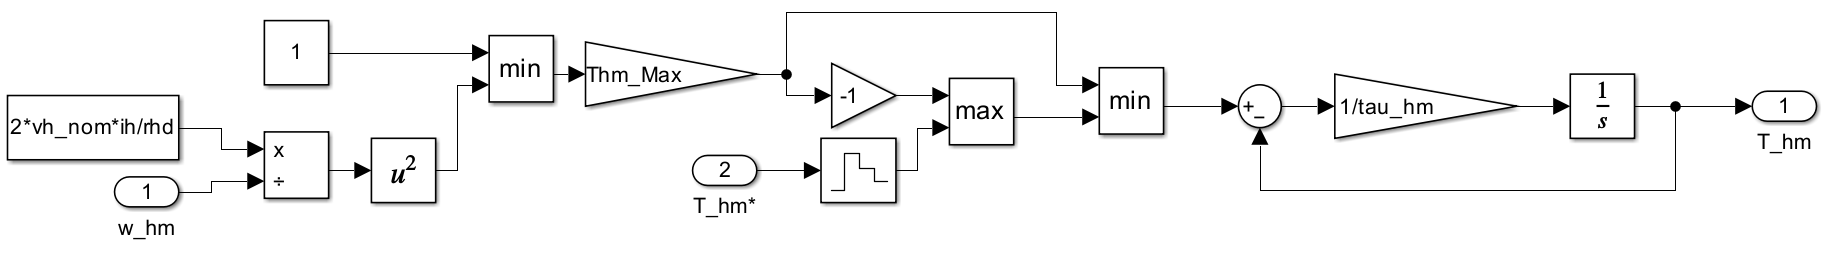
\includegraphics[width=0.72\linewidth]{modulador_izaje.png}
\end{frame}
